\section{Analysis strategy}\label{chap5:analysis_strategy}

\subsection{Event reconstruction}

Regarding the electrons, muons, jets and \MET definition and reconstruction, the standard CMS recommendations described in Chapter~\ref{chap2} are used. The specific selections used in this analysis are briefly summarised below.

Muons are identified according to the CMS recommendations for the medium working point, with the addition of some extra cuts, as defined by the following selections:
\begin{itemize}
\item identified by the standard medium muon selection described in Sec.~\ref{sec:Objects}; \textcolor{red}{Not yet defined :)}
\item $\pt> 10$\GeV;
\item $|\eta < 2.4|$;
\item $|d_{xy}| < 0.01$\,cm for $\pt < 20$\GeV and $|d_{xy}| < 0.02$\,cm for $\pt > 20$\GeV, $d_{xy}$ being the transverse impact parameter with respect to the primary vertex;
\item $|d_{z}| < 0.1$\,cm, where $d_z$ is the longitudinal distance of the muon track in the tracker extrapolated along the beam direction.
\end{itemize}

For the muon isolation, the CMS recommended particle flow isolation based on the tight working point is used, corresponding to a requirement on the isolation variable of $ISO_\mathrm{tight} < 0.15$. In addition a tracker relative isolation is also applied.

For the electron identification, the tight working point is used. In addition some additional cuts to make the selection ``trigger-safe'' are included. This is done because the electron triggers already include some identification and isolation requirements that are based on the raw detector information, while the offline selections make use of particle flow requirements. The ``trigger-safe'' selections are defined to make the the offline identification and isolation requirements tighter with respect to the online triggers.

The simulated events are corrected for the lepton trigger, identification and isolation efficiencies measured in data using the same techniques described in Sec.~\ref{sec:Selections}.

Jets are defined clustering the particle flow objects using the anti-$k_t$ algorithm with a distance parameter of 0.4. The CHS pileup mitigation technique is used. The L1, L2, L3 and L2L3 jet energy correction described in Sec.~\ref{sec:Objects} are applied. The reject jets coming from calorimeter or readout electronics noise, the loose working point for PF jet identification is used.

The b-tagging algorithm for this analysis is chosen comparing the performances of different algorithms using simulations for signal and background contributions in the phase space defined by the analysis kinematic requirements. More precisely, two MC samples are used, one corresponding the the \hwwllnn signal produced via the ggH production mode and another corresponding to the \ttbar process. In fact, the first sample is enriched in light jets, i.e. originating by the hadronization of light quarks like u,d,c and s quarks, while the second sample is enriched in b jets, coming from the top quark decay. The b-veto efficiency, $\epsilon_\mathrm{b veto}$, is computed separately for the two samples and for the various b tagging algorithms. To compare the b tagging performance $\epsilon_\mathrm{b veto}$ is computed for different working points, i.e. different selections on the specific b tagging discriminator, and the results are reported in the form of a ROC curve. The ROC curves corresponding to events with 0, 1 and $\geq 2$ jets are shown in Fig.~\ref{fig:btag}. Events considered for this study are the ones passing the WW baseline selection.

\begin{figure}[!h]
\centering
\subfigure[$N_\mathrm{jets} = 0$]{
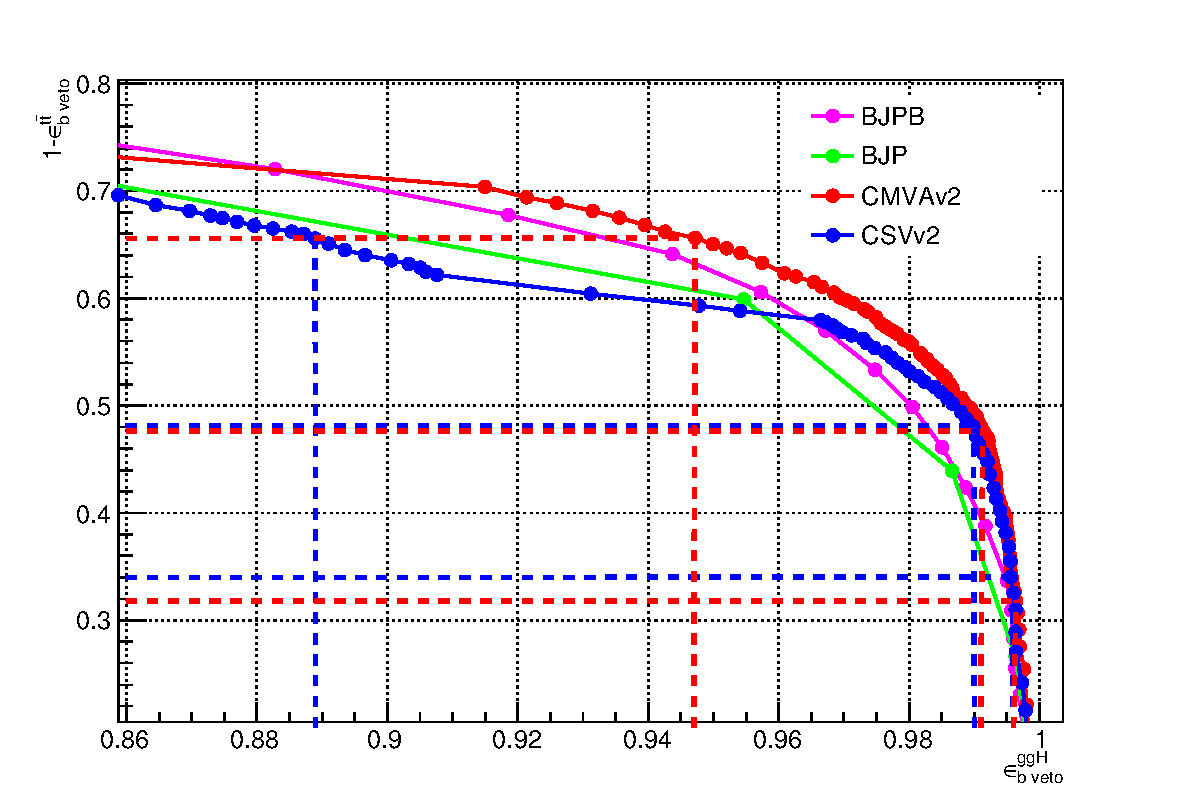
\includegraphics[width=0.45\textwidth]{images/13TeV/ROC_njet0.pdf}
}
\subfigure[$N_\mathrm{jets} = 1$]{
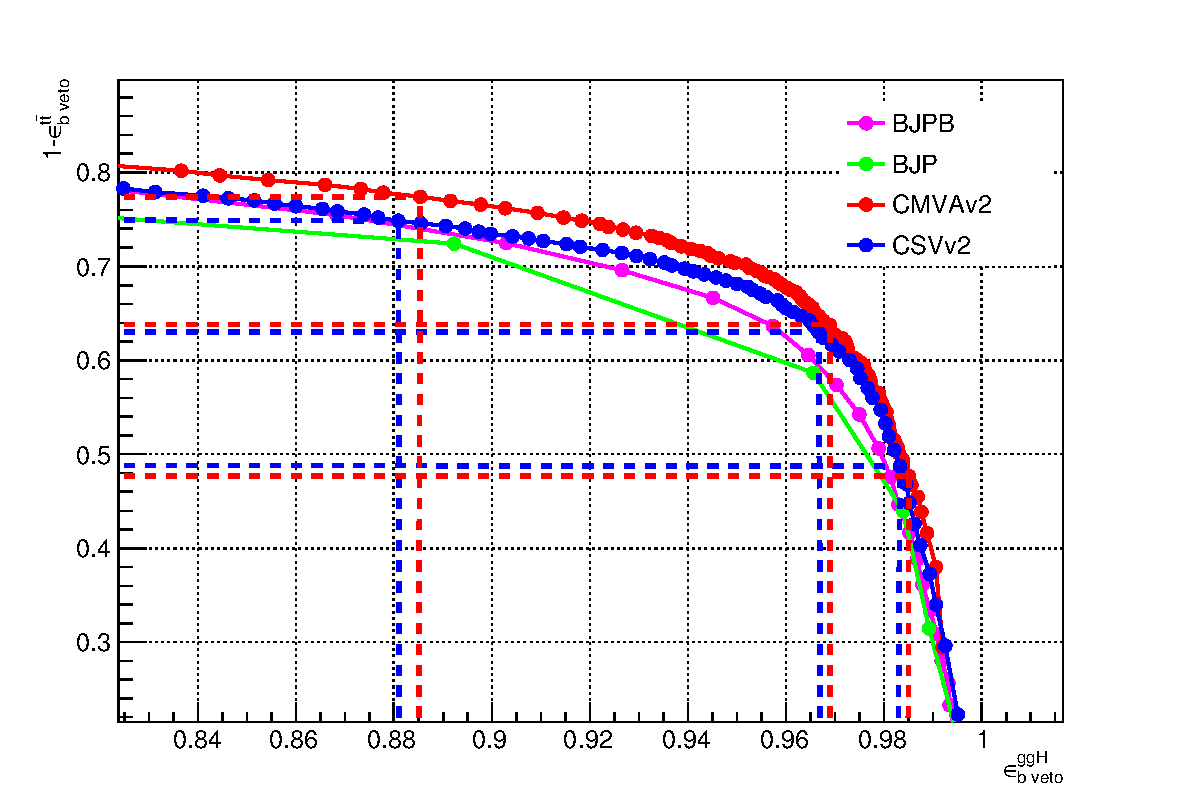
\includegraphics[width=0.45\textwidth]{images/13TeV/ROC_njet1.pdf}
}
\subfigure[$N_\mathrm{jets} \geq 2$]{
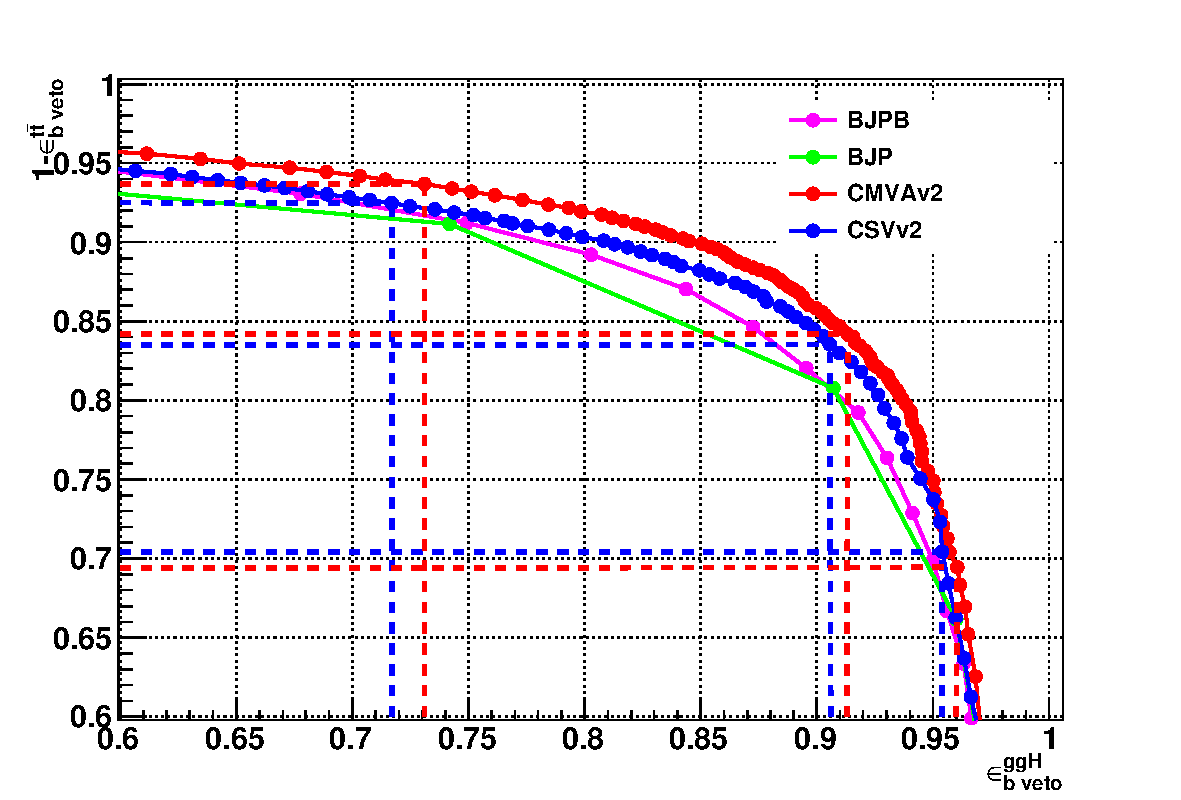
\includegraphics[width=0.45\textwidth]{images/13TeV/ROC_njetge2.pdf}
}
\caption{ROC curve for the b veto efficiency on signal and background events. The blue and red lines point out the signal efficiency and the background rejection corresponding to the three working points considered for the CSVv2 and the cMVAv2 algorithms
respectively.}\label{fig:btag}
\end{figure}

The ROC curves show that the cMVAv2 algorithm has the best performance for the analysis phase space among the algorithms taken into account. For both the CSVv2 and cMVAv2 algorithms, three working points are defined corresponding to the mistag rates\footnote{The mistag rate is defined as the probability for a light jet to be identified as a b-jet by the b tagging algorithms.} of 10\% for the loose, 1\% for the medium and 0.1\% for the tight working point. The distribution of the cMVAv2 discriminator associated to the leading jet both for the ggH and the \ttbar MC sample is shown in figure~\ref{fig:discriminator}.

\begin{figure}[!h]
\centering
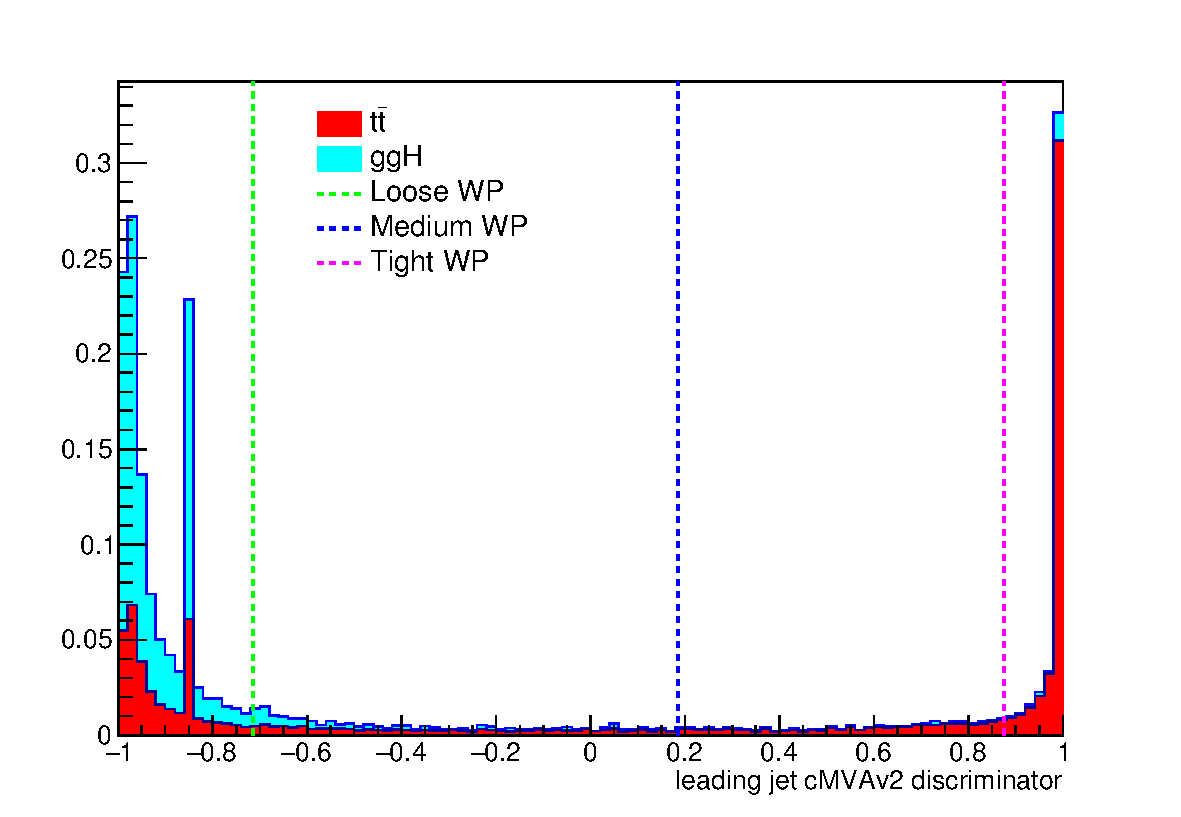
\includegraphics[width=0.8\textwidth]{images/13TeV/cmva_WP.pdf}
\caption{cMVAv2 discriminator associated to the leading jet (with $\pt > 30$~GeV) both for the ggH and the $t\bar t$ processes. The two processes are normalized to unity and stacked. The vertical dashed lines show the discriminator value corresponding to the three working points.}\label{fig:discriminator}
\end{figure}

In order to determine the best working point for this analysis a preliminary significance assessment is performed, using a complete analysis procedure in which only statistical
effects are taken into account (no systematics are included). The significance assessment
was performed using a two dimensional discriminating
variable consisting of the dilepton invariant mass versus the transverse
mass. The assessment was performed with the following leptonic selection:
\begin{itemize}
\item two leptons, an electron and a muon with opposite charge, with
leading lepton \pt greater than 20\GeV and sub-leading lepton \pt greater than
13\GeV;
\item no other lepton (electron or muon) with \pt greated than 10\GeV;
\item \mll greater than 12\GeV;
\item PF type 1 corrected MET greater than 20\GeV;
\item \ptll greater than 30\GeV.
\end{itemize}
In addition to this global selection, two categories were identified:
\begin{itemize}
\item 0 jets: no jets above 30\GeV, jets between 20\GeV and 30\GeV are
b-vetoed with the cMVAv2 WP under study;
\item 1 jet: exactly 1 jet above 30\GeV, no b-tagged jets above 30\GeV
according to the cMVAv2 WP under study.
\end{itemize}
The two categories were eventually combined together and the significance 
assessment was repeated for the three working points.
With these selection we find the significance values listed in
Table~\ref{tab:significance_wp_combine} for the three working points.
\begin{table}
\caption{Significance corresponding to the three working points and for
different jet categories using a shape
analysis.\label{tab:significance_wp_combine}}
\begin{center}
\begin{tabular}{cccc}
\toprule
Jet category & Loose WP (-0.715) & Medium WP (0.185) & Tight WP (0.875) \\
\midrule
0 jets & 2.022 & 2.043 & 2.036 \\
1 jet & 1.439 & 1.404 & 1.305 \\
$0+1$ jets & 2.481 & 2.479 & 2.420 \\
\bottomrule
\end{tabular}
\end{center}
\end{table}

The working point providing the best significance in the combined $0+1$ jets category is found to be the loose one.

To correct for a possible different b tagging efficiency in data and simulation, the simulated events are reweighted using scale factors computed in bins of the jet $\eta$ and \pt. These scale factors and the corresponding uncertainties are centrally calculated for each working point, in such a way to be employable by all the CMS analyses. The prescription to reweight the simulated events is the following. First of all one has to compute the b tagging efficiency using the MC samples, $\varepsilon_\mathrm{MC}(p_\mathrm{T}, \eta, f)$, for the chosen working point in bins of jet \pt and $\eta$. The efficiency has to be computed for different flavours $f$ of the jets, b, c and light (u,d,s), using the jet matching information\footnote{There are a couple of techniques developed by the CMS Collaboration to assess the flavour of a reconstructed jet in simulation. The technique used here makes use of the flavour of the hadrons clustered into a jet.} which is available in all the MC samples. An MC-based event weight is then calculated computing the probability $P_\mathrm{MC}$ of a given b tagging configuration to occur, e.g.:
\begin{equation}
P_\mathrm{MC}=\prod_{i~\in{}~b-tagged-jets}\varepsilon_{\mathrm{MC}_{i}}\prod_{j~\in{}~non-b-tagged-jets}(1-\varepsilon_{\mathrm{MC}_{j}})
\label{eq:btagpmc}
\end{equation}
Afterwards, a similar probability is computed using data:
\begin{equation}
P_\mathrm{DATA}=\prod_{i~\in{}~b-tagged-jets}SF_{i}\varepsilon_{\mathrm{MC}_{i}}\prod_{j~\in{}~non-b-tagged-jets}(1-SF_{j}\varepsilon_{\mathrm{MC}_{j}}) \quad ,
\label{eq:btagpdata}
\end{equation}
where $SF_{i}$ is the provided scale factor value for the relevant jet flavour, \pt and $\eta$. Products in Eqs.~\ref{eq:btagpmc} and \ref{eq:btagpdata} run over all jets. The event weight is finally given by the ration $P_\mathrm{DATA}/P_\mathrm{MC}$.

The b tagging efficiencies to be fed into Eq.~\ref{eq:btagpmc} and
Eq.~\ref{eq:btagpdata} are derived using \ttbar simulated events and applying basic leptonic
selections. These efficiencies are shown in Fig.~\ref{fig:effmc} for light
(a), c-jets (b) and b-jets (c), in bins of $\eta$ and \pt. The uncertainties associated to the efficiencies are representative of the statistics of the simulated \ttbar sample, and are computed according to a binomial distribution.
\begin{figure}[!h]
\centering
\subfigure[]{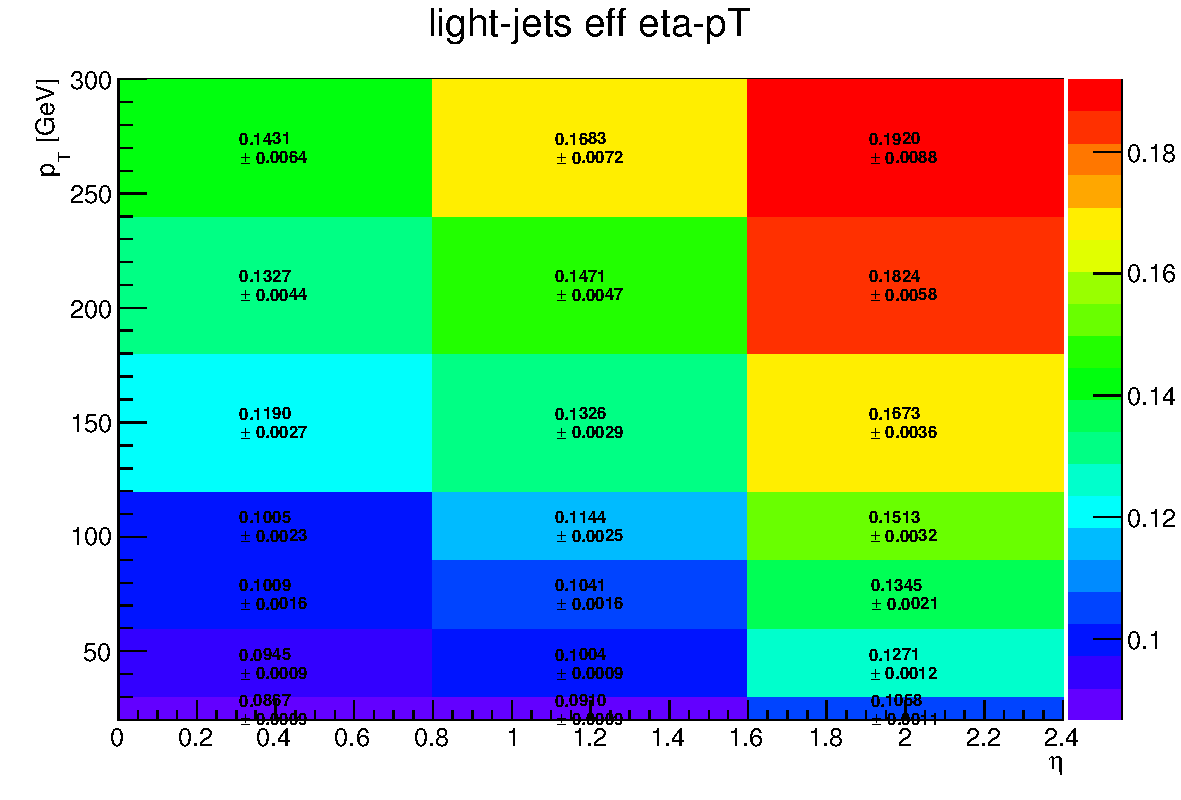
\includegraphics[width=0.4\textwidth]{images/13TeV/ljet_effmc.pdf}}
\subfigure[]{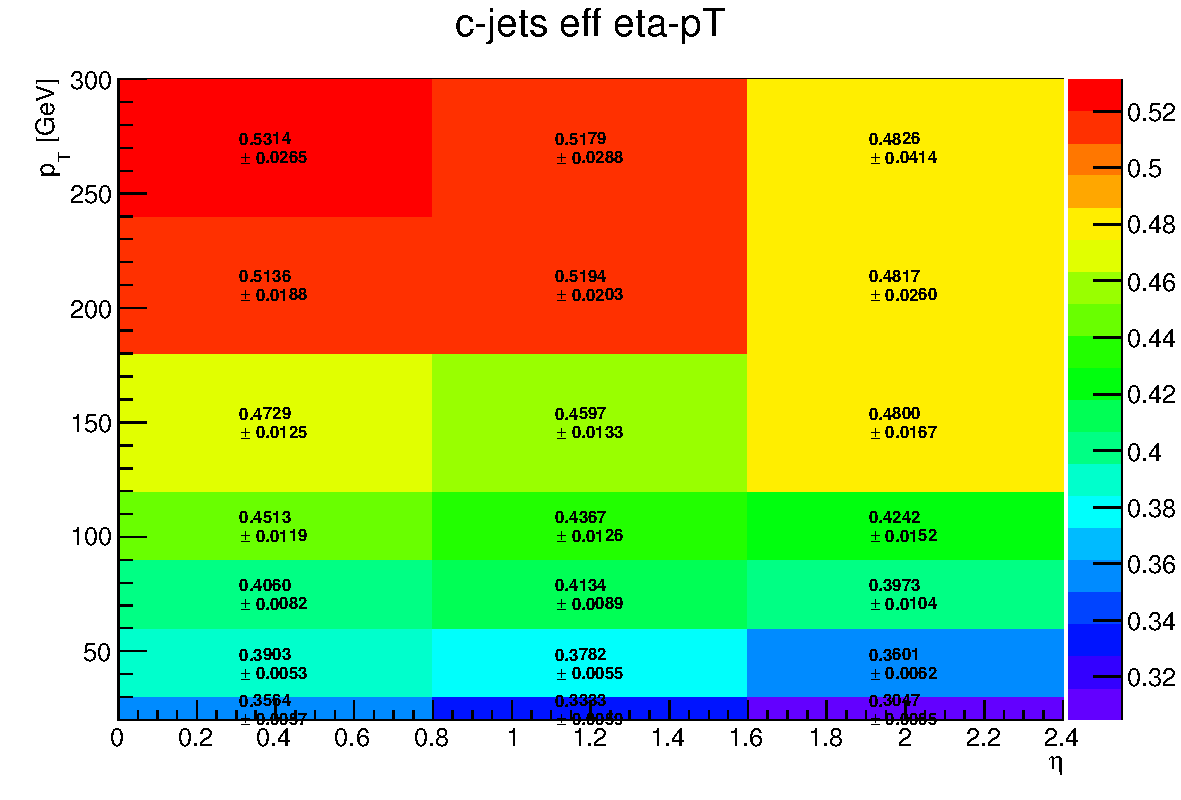
\includegraphics[width=0.4\textwidth]{images/13TeV/cjet_effmc.pdf}}\\
\subfigure[]{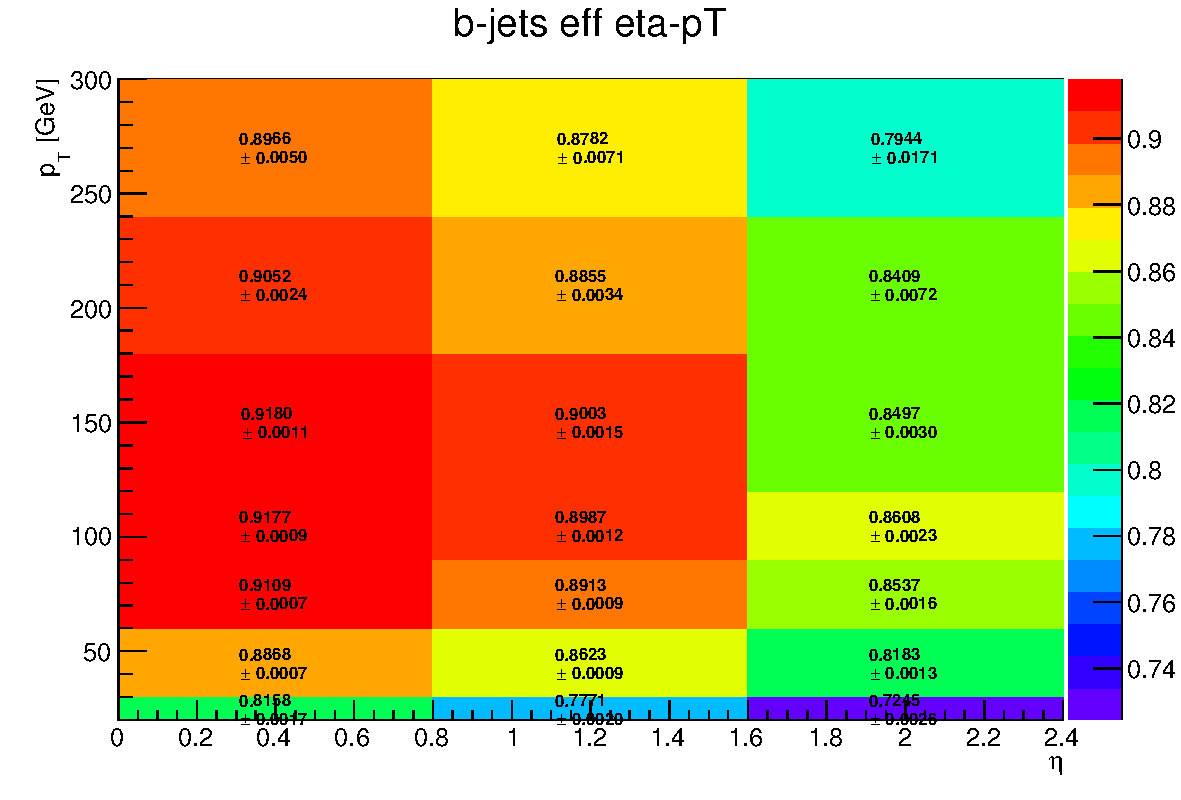
\includegraphics[width=0.4\textwidth]{images/13TeV/bjet_effmc.pdf}}
\caption{B tagging efficiencies for light jets (a), c-jets (b) and
b jets (c), as a function of $\eta$ and \pt.\label{fig:effmc}}
\end{figure}


The effect of the event reweighting is to correct the shape of the b tagging discriminator in simulation, moving events from the b tag region (discriminator greater than $> -0.715$) to the b veto region (discriminator $ < -0.715$) and viceversa. A data/simulation comparison of the b tagging discriminator for the leading and subleading jets is performed to check the agreement after the application of the event weights. In order to evaluate the data/simulation agreement for b-jets, the data and simulation are compared in a top enriched control region, defined by the following requirements:
\begin{itemize}
\item two leptons, an electron and a muon with opposite charge, with
leading lepton \pt greater than 20\GeV and sub-leading lepton \pt greater than
15\GeV;
\item no other lepton (electron or muon) with \pt greater than 10\GeV;
\item lepton invariant mass greater than 50\GeV;
\item at least two jets with \pt greater than 30 GeV;
\item at least one of the two leading jets with cMVAv2 btagging score
greater than -0.715 (i.e. the loose working point).
\end{itemize}
In order to evaluate the agreement for light jets, a second
control region is defined, populated by Z+light jet events, defined as follows:
\begin{itemize}
\item two leptons, two electrons or two muons with opposite charge, with
leading lepton \pt greater than 20\GeV and sub-leading lepton \pt greater than
15\GeV.
\item no other lepton (electron or muon) with \pt greater than 10\GeV.
\item lepton invariant mass greater between 80\GeV and 110\GeV.
\item at least two jets with \pt greater than 30 GeV.
\item at least one jet above 30\GeV.
\item no jets above 20\GeV with a TCHE score above 2.1. 
\end{itemize}
Although a Z+jets sample is dominated by light flavor jets, a b-veto on an
alternative algorithm (TCHE) is applied to reduce the contamination from b-jets,
especially above the cMVAv2 cut.  This helps mitigating possible data/simulation discrepancies in the modeling of the heavy/light flavour ratio.
The comparison between data and simulation after the event reweighting is shown in Figs.~\ref{fig:bpogSF} and \ref{fig:bpogSF_Z} for the b-jets and light jets enriched control regions, respectively.

\begin{figure}[!h]
\centering
\subfigure[]{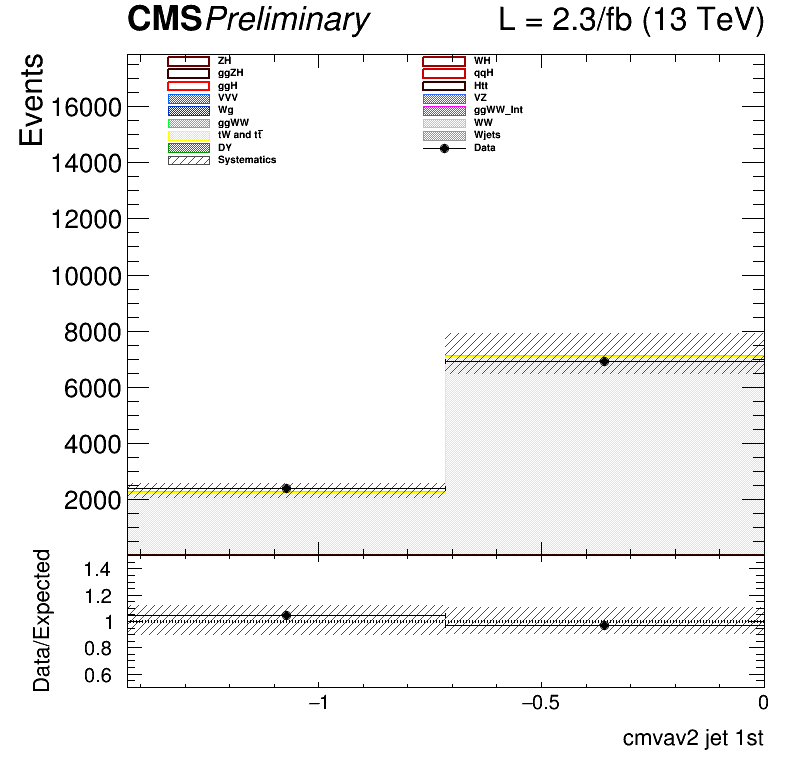
\includegraphics[width=0.4\textwidth]{images/13TeV/cratio_hww2l2v_13TeV_top_of1j_cmva_twobins_1.png}}
\subfigure[]{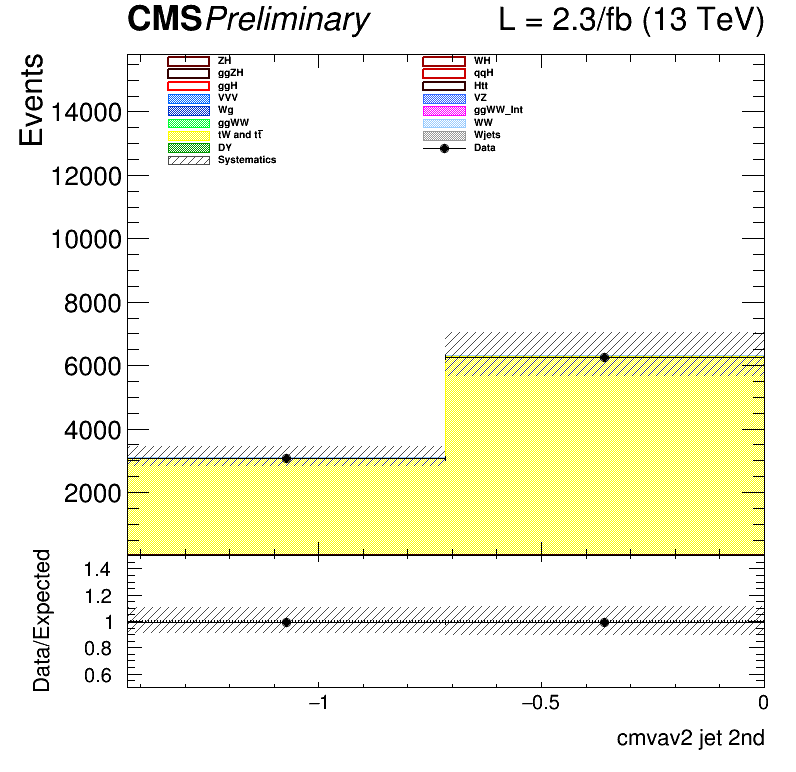
\includegraphics[width=0.4\textwidth]{images/13TeV/cratio_hww2l2v_13TeV_top_of1j_cmva_twobins_2.png}}
\caption{B tagging cMVAv2 discriminator for the leading (a) and the subleading (b)
jet in the b-jets enriched control region.\label{fig:bpogSF}}
\end{figure}
\begin{figure}[!h]
\centering
\subfigure[]{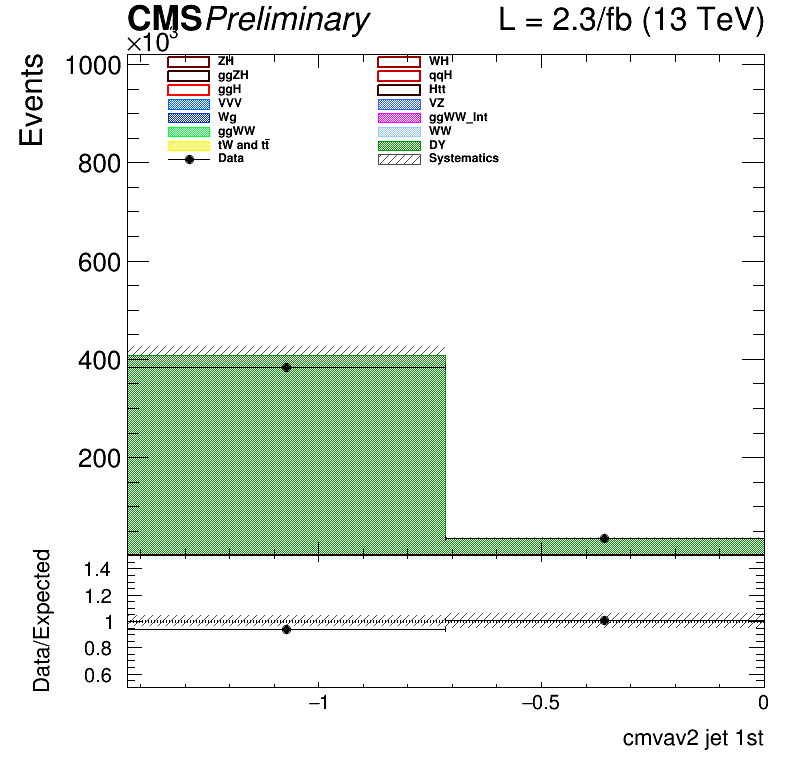
\includegraphics[width=0.4\textwidth]{images/13TeV/cratio_ZjetsCutTCHE_mumu_cmva_twobins_1.png}}
\subfigure[]{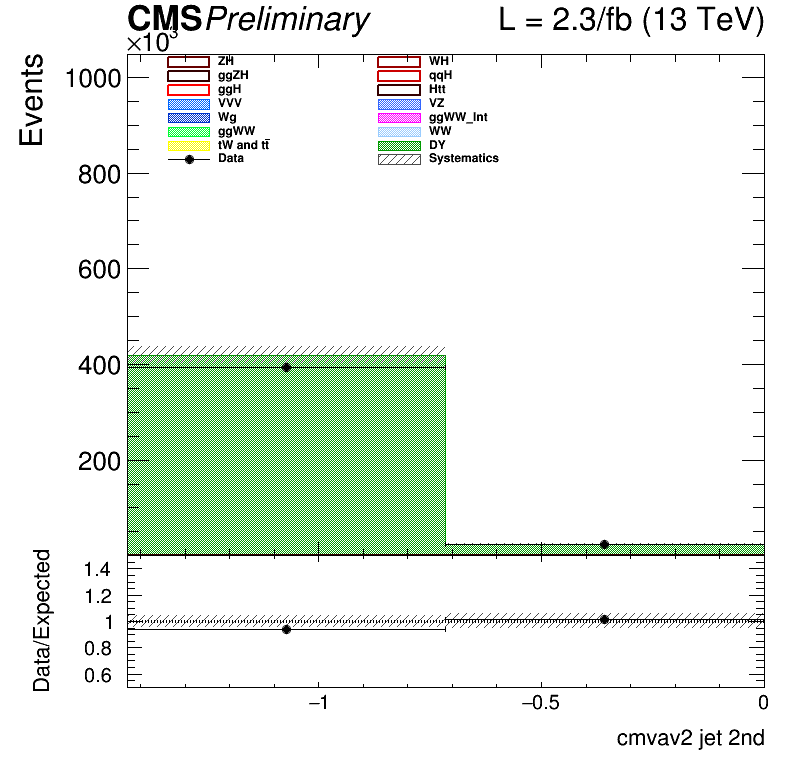
\includegraphics[width=0.4\textwidth]{images/13TeV/cratio_ZjetsCutTCHE_mumu_cmva_twobins_2.png}}
\caption{B tagging cMVAv2 discriminator for the leading (a) and the subleading (b)
jet in the light jets enriched control region.\label{fig:bpogSF_Z}}
\end{figure}

\subsection{Event selection and background rejection}\label{chap5:eventSel}

Since the ggH production mechanism, which is the main production mode for a Higgs mass of around 125\GeV, is characterized by the emission of few jets arising from initial or final state radiation, this analysis is limited to events with no jets or one jet. Due to the large DY background in di-electrons and di-muons events, only the $e\mu$ final state is studied in this early Run 2 data analysis, including the indirect contribution from $\tau$ leptons decaying to electron or muons.
Exactly one electron and one muon are required to be reconstructed in the event with opposite charges and a minimum \pt of 10 (13)\GeV for  the muon (electron). One of the two leptons should also have a \pt greater than 20\GeV and both leptons are required to be well identified and isolated to reject fake leptons and leptons coming from QCD sources. To suppress background processes with three or more leptons in the final state, such as ZZ, WZ, Z$\gamma$, W$\gamma$, or tri-boson production, no additional identified and isolated lepton with $\pt>10$\GeV should be reconstructed. The low \mll region dominated by QCD production of leptons
is not considered in the analysis and \mll is requested to be higher than 12\GeV. To suppress the background arising from DY events decaying to a $\tau$ lepton pair which subsequently
decays to an $e\mu$ final state and suppress processes without genuine \MET, a minimal \MET of 20\GeV
is required. The DY background is further reduced by requesting $\ptll > 30$\GeV.
 Finally the contribution from leptonic decays of single top and \ttbar production is reduced by requesting
that no jets with $\pt>20$\GeV are identified by the b tagging algorithm as originating from a b quark in the event.

The requirements described above define the WW baseline selection. After those requirements the data sample is dominated by events arising from the non-resonant WW production and \ttbar production. To further reduce the effect of these backgrounds on the signal sensitivity, the events are categorized depending on the jet multiplicity, counting jets with $\pt > 30$\GeV. Events with zero associated jets mainly arise from the WW production, while WW and \ttbar productions have a similar contribution in the category with one jet. Higher jet multiplicity categories, which are sensitive to other Higgs production mechanisms, such as VBF, are not included in this analysis, given the very low expected yield for other production modes with the analysed integrated luminosity.

Distributions of some variables of interest for the 0 and 1 jet categories separately, but merging the e$\mu$ and $\mu$e final states together, are shown in Figs.~\ref{fig:distr1}, \ref{fig:distr2} and \ref{fig:distr3} after applying the WW baseline selections, with the addition of a cut on \mll to remove the Higgs signal contribution ($\mll > 80$\GeV), and a cut on \mt to be orthogonal to the $\mathrm{Z}\gamma^* \to \tau\tau$ background control region ($\mt > 60$\GeV).

\begin{figure}
\centering
\subfigure[0 jets - $\pt^{\ell,1}$]{
  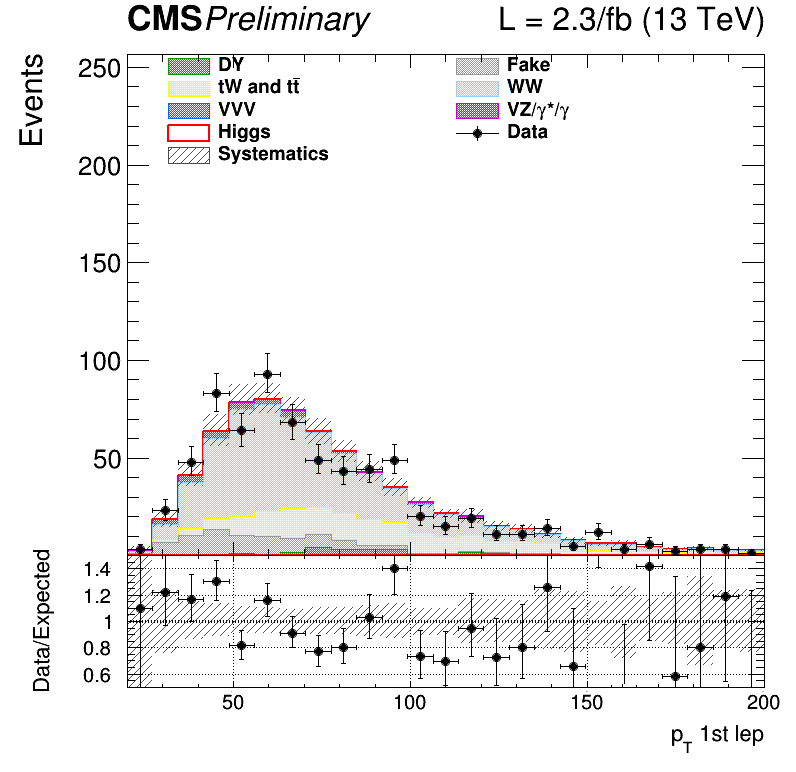
\includegraphics[width=0.45\textwidth]{images/13TeV/cratio_ww2l2v_13TeV_ww_of0j_pt1}
}
\subfigure[0 jets - $\eta^{\ell,1}$]{
  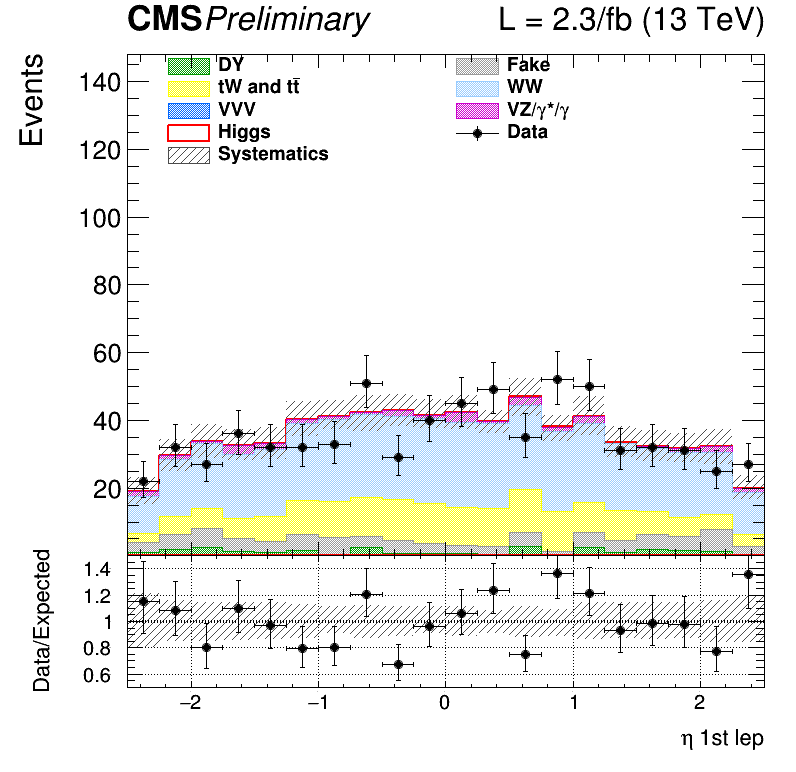
\includegraphics[width=0.45\textwidth]{images/13TeV/cratio_ww2l2v_13TeV_ww_of0j_eta1}
}\\
\subfigure[1 jet - $\pt^{\ell,1}$]{
  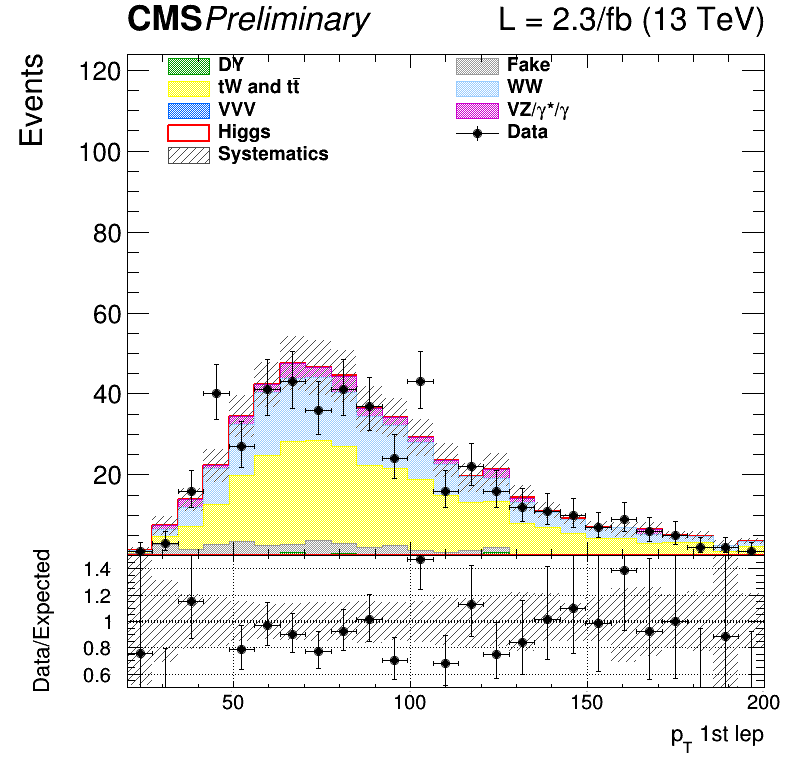
\includegraphics[width=0.45\textwidth]{images/13TeV/cratio_ww2l2v_13TeV_ww_of1j_pt1}
}
\subfigure[1 jet - $\eta^{\ell,1}$]{
  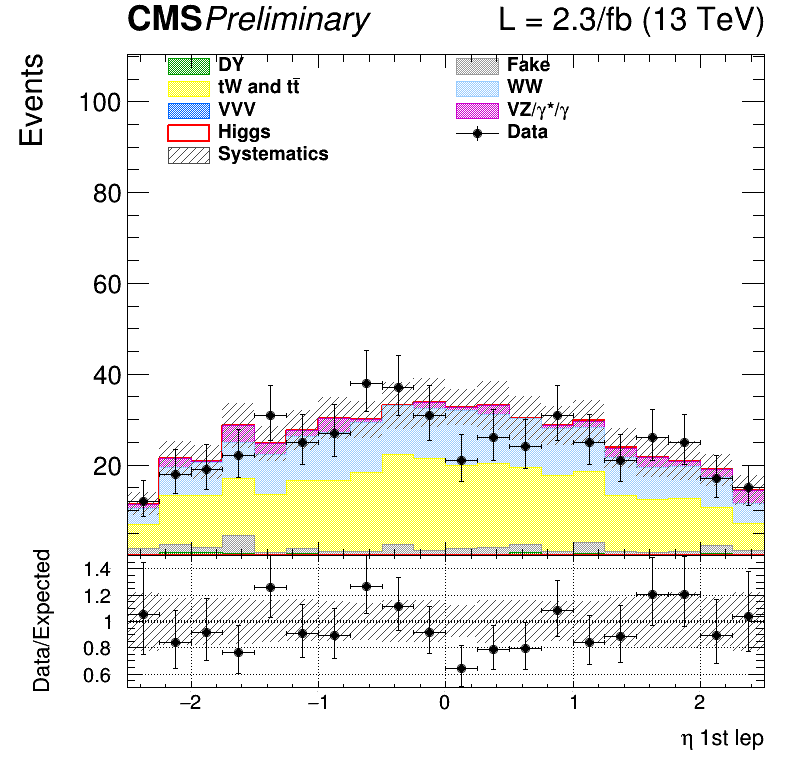
\includegraphics[width=0.45\textwidth]{images/13TeV/cratio_ww2l2v_13TeV_ww_of1j_eta1}
}
\caption{Distributions of \pt (left) and $\eta$ (right) of the leading lepton for events with 0 jet (upper row) and 1 jet (lower row), for the main backgrounds (stacked histograms), and for a SM Higgs boson signal with $m_\mathrm{H}=125$\GeV (superimposed and stacked red histogram) at the WW selection level. The last bin of the histograms includes overflows. The simulation of the WW background is normalized to data.}\label{fig:distr1}
\end{figure}

\begin{figure}
\centering
\subfigure[0 jets - $\pt^{\ell,2}$]{
  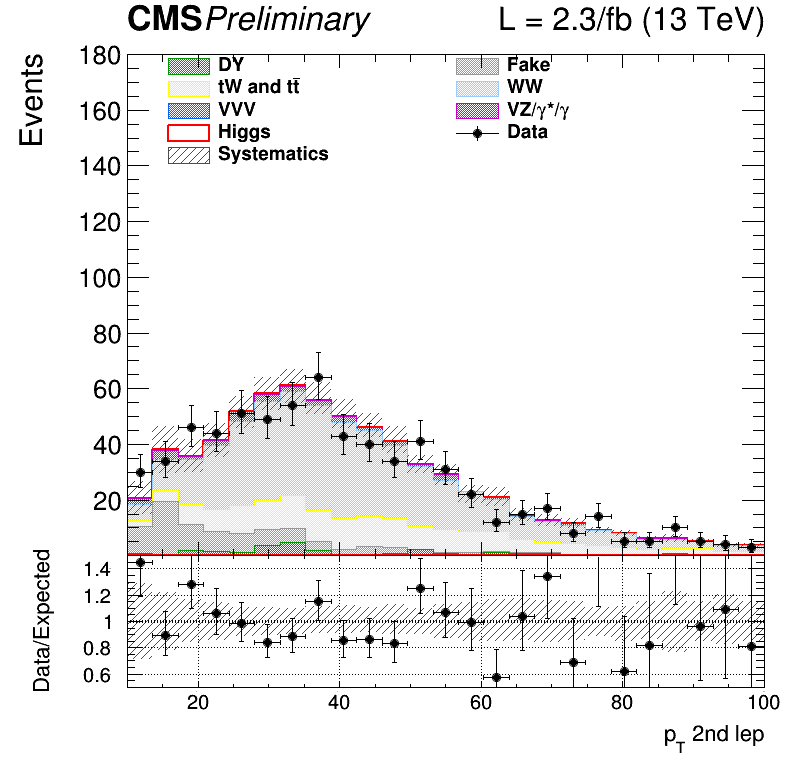
\includegraphics[width=0.45\textwidth]{images/13TeV/cratio_ww2l2v_13TeV_ww_of0j_pt2}
}
\subfigure[0 jets - $\eta^{\ell,2}$]{
  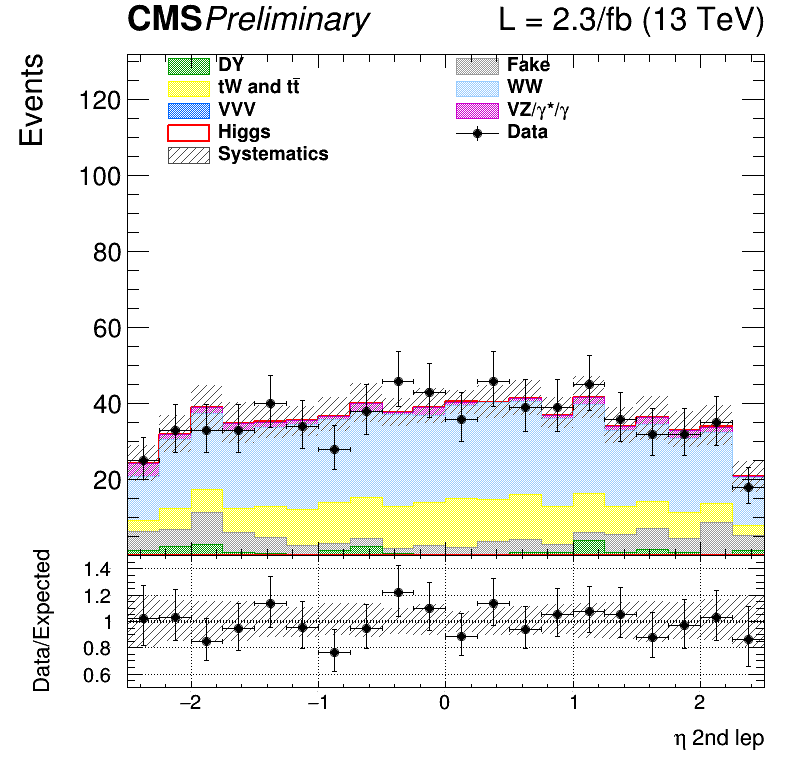
\includegraphics[width=0.45\textwidth]{images/13TeV/cratio_ww2l2v_13TeV_ww_of0j_eta2}
}\\
\subfigure[1 jet - $\pt^{\ell,2}$]{
  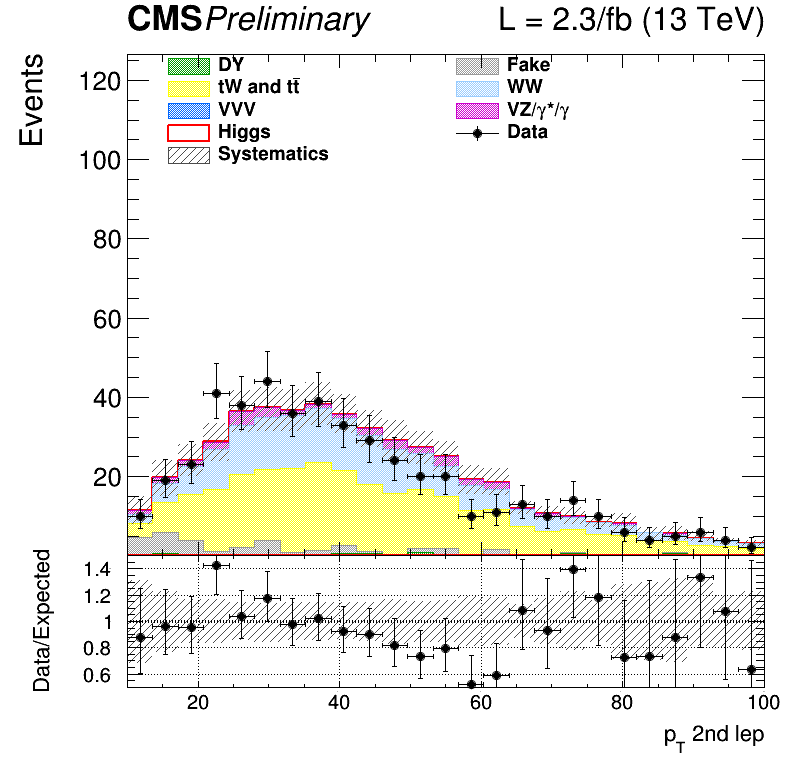
\includegraphics[width=0.45\textwidth]{images/13TeV/cratio_ww2l2v_13TeV_ww_of1j_pt2}
}
\subfigure[1 jet - $\eta^{\ell,2}$]{
  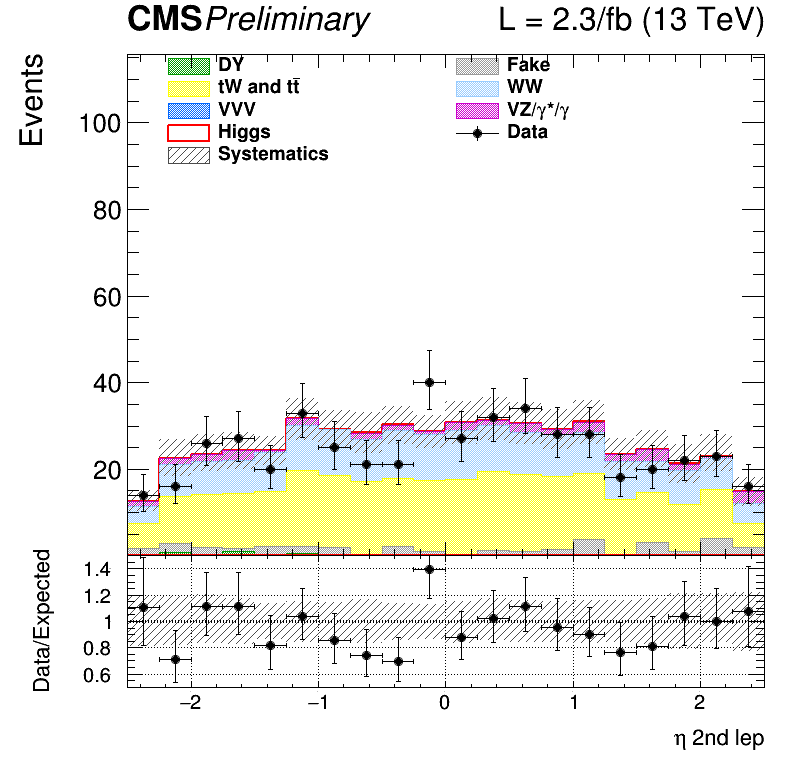
\includegraphics[width=0.45\textwidth]{images/13TeV/cratio_ww2l2v_13TeV_ww_of1j_eta2}
}
\caption{Distributions of \pt (left) and $\eta$ (right) of the subleading lepton for events with 0 jets (upper row) and 1 jet (lower row), for the main backgrounds (stacked histograms), and for a SM Higgs boson signal with $m_\mathrm{H}=125$\GeV (superimposed and stacked red histogram) at the WW selection level. The last bin of the histograms includes overflows. The simulation of the WW background is normalized to data.}\label{fig:distr2}
\end{figure}

\begin{figure}
\centering
\subfigure[0 jets - \MET]{
  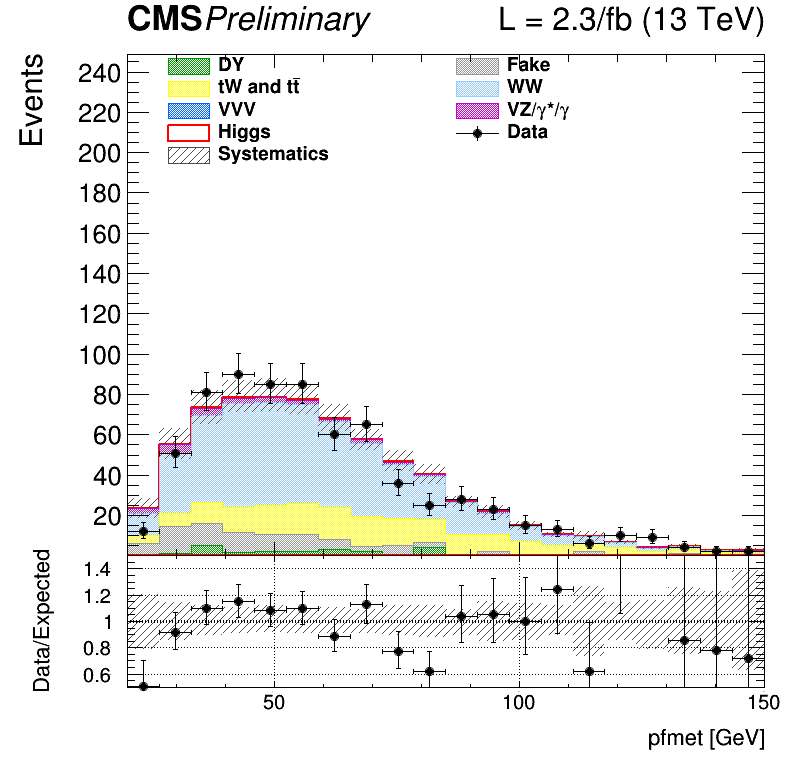
\includegraphics[width=0.45\textwidth]{images/13TeV/cratio_ww2l2v_13TeV_ww_of0j_met}
}
\subfigure[0 jets - \ptll]{
  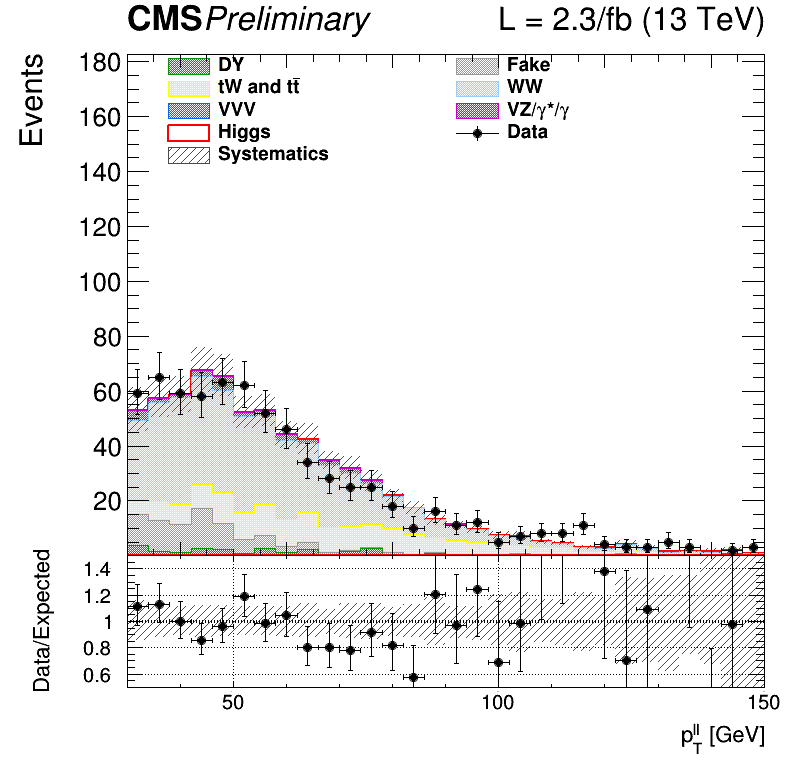
\includegraphics[width=0.45\textwidth]{images/13TeV/cratio_ww2l2v_13TeV_ww_of0j_ptll}
}\\
\subfigure[1 jet - \MET]{
  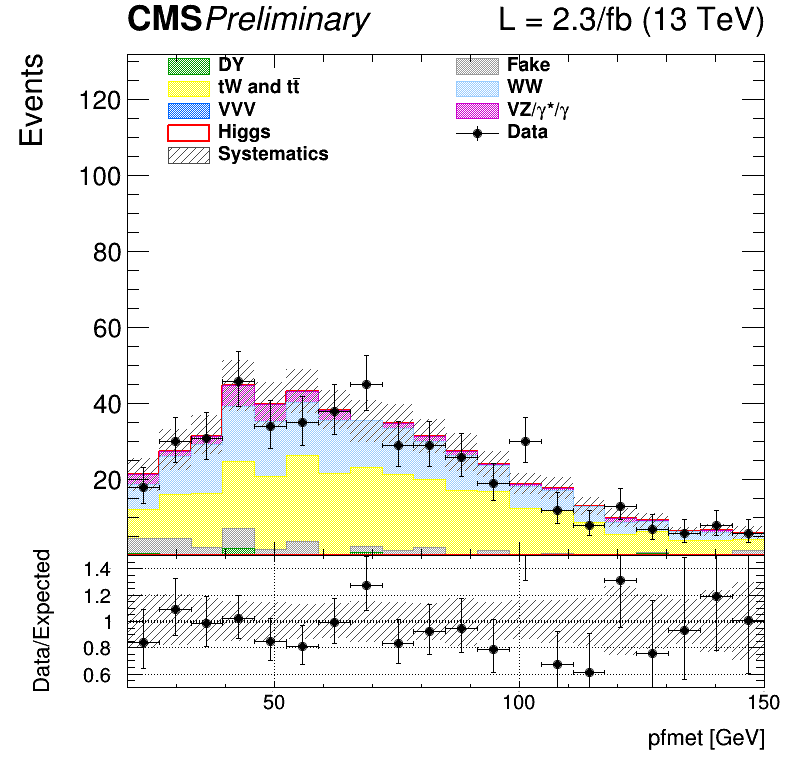
\includegraphics[width=0.45\textwidth]{images/13TeV/cratio_ww2l2v_13TeV_ww_of1j_met}
}
\subfigure[1 jet - \ptll]{
  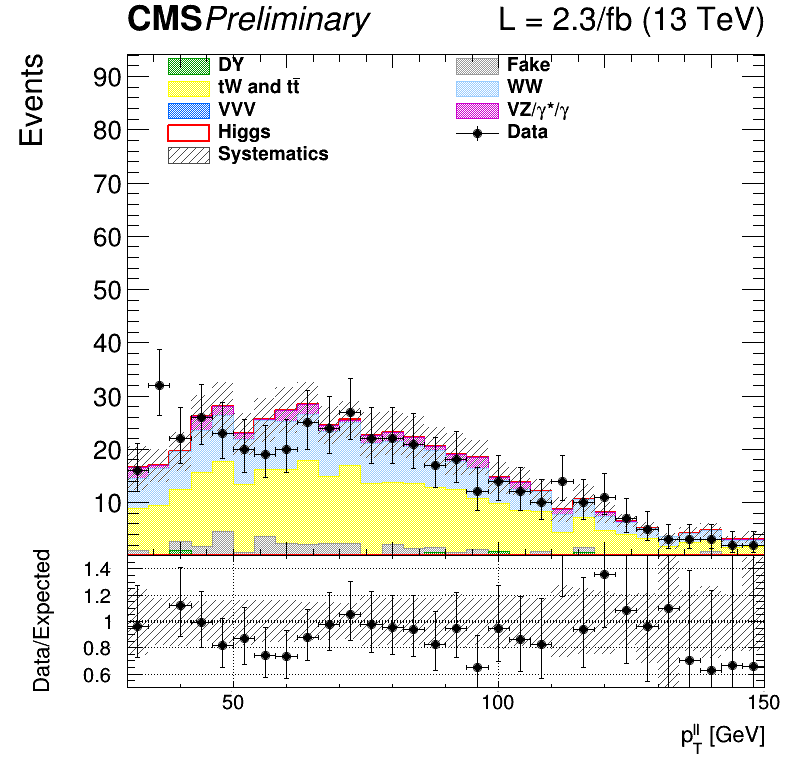
\includegraphics[width=0.45\textwidth]{images/13TeV/cratio_ww2l2v_13TeV_ww_of1j_ptll}
}
\caption{Distributions of \MET (left) and \ptll (right) for events with 0 jets (upper row) and 1 jet (lower row), for the main backgrounds (stacked histograms), and for a SM Higgs boson signal with $m_\mathrm{H}=125$\GeV (superimposed and stacked red histogram) at the WW selection level. The last bin of the histograms includes overflows. The simulation of the WW background is normalized to data.}\label{fig:distr3}
\end{figure}

The W+jets background, where one jet can be misidentified as a lepton, is a sub-dominant background in the phase space defined by the analysis kinematic requirements. The 0 ad 1 jets categories are further split according to the lepton flavour to e$\mu$ and $\mu$e, where the first lepton refers to the leading one. In this way an improvement of about 10\% in terms of the signal significance can be achieved, exploiting the different W+jets background contribution in the two categories. Indeed the probability for a jet to be misidentified as an electron or a muon is not the same.



\subsection{Signal extraction}

To extract the Higgs boson signal contribution in the four previously mentioned categories, a similar approach to the one used in the Run 1 analysis~\cite{Chatrchyan:2013iaa} is pursued. The analysis is based on two-dimensional templates of \mll versus \mt to discriminate signal and background contributions. The \mll template is defined using 5 bins from $\mll=10$\GeV up to $\mll=110$\GeV, while for the \mt template 7 bins are defined in the range $60\GeV < \mt < 200$\GeV. The phase space with $\mt<60$\GeV is used as an orthogonal control region to extract the normalization of the DY background. A binned maximum likelihood fit to the signal and background two-dimensional templates is performed to extract the signal strength in the four categories.

Distributions of the \mll and \mt variables after the WW level selection are shown in Fig.~\ref{fig:mllandmt} for the 0 and 1 jet categories separately, but merging the e$\mu$ and $\mu$e final states together.

\begin{figure}
\centering
\subfigure[0 jets - \mll]{
  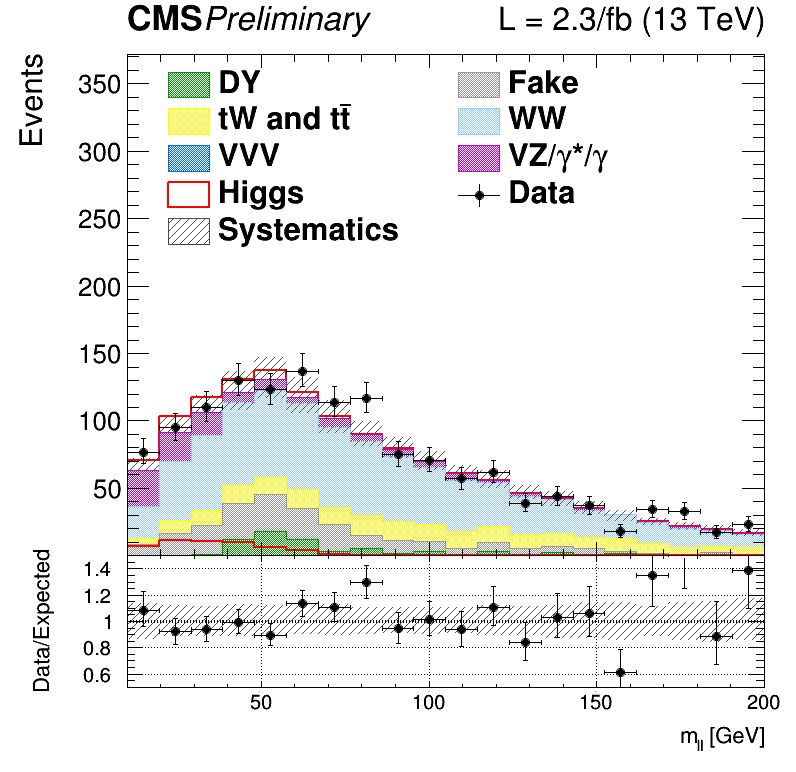
\includegraphics[width=0.45\textwidth]{images/13TeV/cratio_hww2l2v_13TeV_of0j_mll}
}
\subfigure[0 jets - \mt]{
  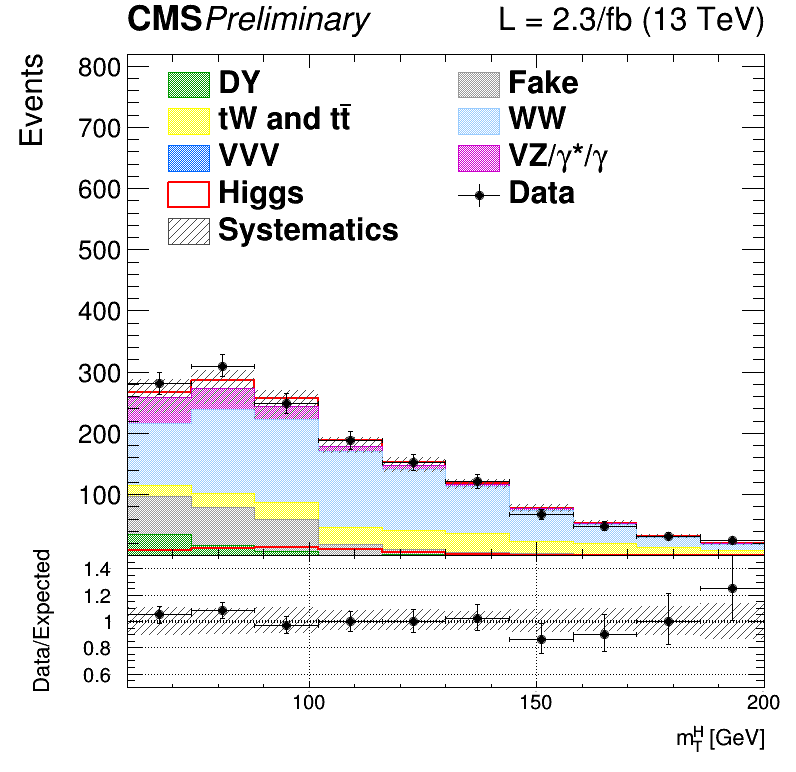
\includegraphics[width=0.45\textwidth]{images/13TeV/cratio_hww2l2v_13TeV_of0j_mth}
}\\
\subfigure[1 jet - \mll]{
  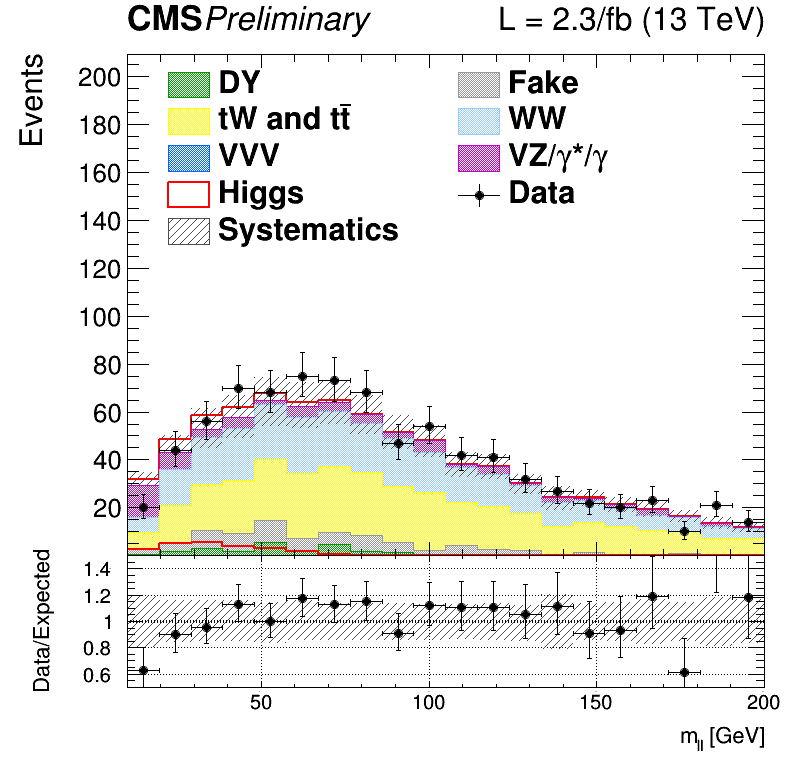
\includegraphics[width=0.45\textwidth]{images/13TeV/cratio_hww2l2v_13TeV_of1j_mll}
}
\subfigure[1 jet - \mt]{
  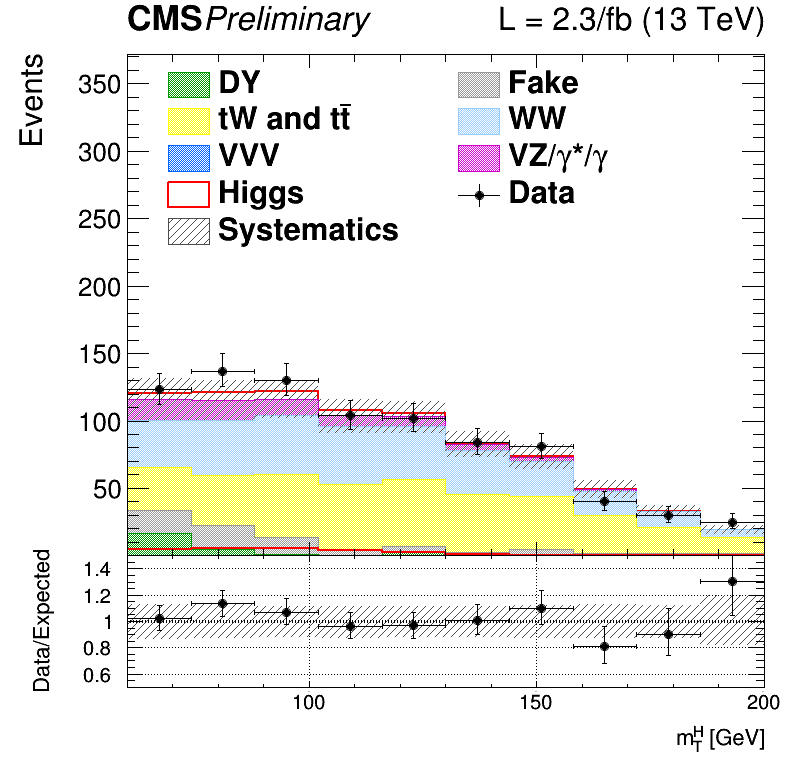
\includegraphics[width=0.45\textwidth]{images/13TeV/cratio_hww2l2v_13TeV_of1j_mth}
}
\caption{Distributions of \mll (left) and \mt (right) for events with 0 jets (upper row) and 1 jet (lower row), for the main backgrounds (stacked histograms), and for a SM Higgs boson signal with $m_\mathrm{H}=125$\GeV (superimposed and stacked red histogram) at the WW selection level. The last bin of the histograms includes overflows. The simulation of the WW background is normalized to data.}\label{fig:mllandmt}
\end{figure}

The statistical methodology used to interpret the data and to combine the results from the independent 0-jet and 1-jet categories in the e$\mu$ and $\mu$e final states has been developed by the ATLAS and CMS collaborations in the context of the LHC Higgs Combination Group~\cite{CMS-NOTE-2011-005,Khachatryan:2014jba}.
The number of events in each category and in each bin of two-dimensional template is modelled as a Poisson random variable,
with a mean value given by the sum of the contributions from all the processes under consideration.
Systematic uncertainties are represented by individual nuisance parameters
with log-normal distributions. The uncertainties affect the overall
normalization of the signal and backgrounds
as well as the shape of the predictions across the distribution of the observables.
Correlation between systematic uncertainties in different categories 
are taken into account. 












